\documentclass{plantillaPPT}

\titulo{3}{Sumas Superior e Inferior}

\begin{document}
\primeraDiapo

\begin{frame}{Integral Indefinidas}
    \framesubtitle{Práctica 3}

1. Calcule la siguiente integral indefinida:

\[\int \sqrt{e^x-1}dx\]
    
\end{frame}

\begin{frame}{Obtención de fórmula de integración}
    \framesubtitle{Práctica 3}
    \vspace{-1cm}

2. Sea \(f: A\subset \mathbb{R} \to \mathbb{R}\) la función definida por: \vspace{0.25cm}
\[f(x) = \frac{1}{x-x^{\alpha+1}}\; , \quad \text{con }  \alpha \in \mathbb{R} - \{-1, 0\}\]
\vspace{0.25cm}

\hspace{-0.5cm}\((a)\) Calcule \(\int f(x)dx\) haciendo el uso del cambio de variable: \(u = x^\alpha\). \\
\hspace{-0.5cm}\((b)\) Utilice lo obtenido en el ítem anterior para calcular: \(\int \frac{1}{x-x^{11}}dx\).
    
\end{frame}

\begin{frame}{Suma superior e inferior}
    \framesubtitle{Práctica 3}
    \vspace{-1cm}
3. Sea \(f: [-4,2] \to \mathbb{R}\) la función definida por:
\vspace{0.25cm}
\[f(x) = \begin{cases}
    \; 1+x & \quad \text{si } -4\leq x <-1 \\
    \; 1-x^2 & \quad \text{si } -1\leq x \leq 2
\end{cases}\]
\vspace{0.25cm}
Determine el valor de la suma superior e inferior de \(f\) con respecto \\ \vspace{-0.2cm} a la partición regular P que divide al intervalo \([-4,2]\) en 6 subintervalos.

\end{frame}

\begin{frame}{Definición de partición}
    \framesubtitle{Suma superior e inferior}

\begin{definicion}
Sean \(a,b \in \mathbb{R}\) con \(a<b\). Una \textit{partición del intervalo} \([a,b]\), es un conjunto \vspace{0.25cm}
\[P = \{x_0, x_1,..., x_n\}\] \\
\vspace{0.25cm}
de \(n+1\) puntos tales que \(a=x_0<x_1<...<x_n=b\)
\end{definicion}
    
\end{frame}

\begin{frame}{Máximos y mínimos de cada sub-intervalo}
    \framesubtitle{Suma superior e inferior}

\begin{definicion}
    Sea \([a,b]\) un intervalo real. Sea \(P\) una partición de él, e \(I_k\) los \\ \vspace{0.1cm} subintervalos correspondientes a \(P\). \\ \vspace{0.15cm} Si \(f : [a,b] \to \mathbb{R}\) es una función continua, el teorema de valores \\ \vspace{0.1cm}extremos nos permite fijar

    \[m_k := \inf\{f(x):x\in[x_{k-1},x_k]\}\]
    \[M_k := \sup\{f(x):x\in[x_{k-1}, x_k]\}\]
\end{definicion}
    
\end{frame}

\begin{frame}{Suma superior e inferior}
    \framesubtitle{Definición}

    \begin{definicion}
        Sea \([a,b]\) un intervalo real. Sea P una partición de él y \(f : [a,b] \to \mathbb{R}\) continua.
        \begin{itemize}
            \item La \textbf{suma inferior} de \(f\) asociada a la partición \(P\) es:
            \[\underline{S}(f,P) := \sum_{k=1}^n m_k \cdot \Delta k\]
            \item La \textbf{suma superior} de \(f\) asociada a la partición \(P\) es:
            \[\overline{S}(f,P) := \sum_{k=1}^n M_k \cdot \Delta k\] \\ \vspace{0.25cm}
            Con \(\Delta k = x_k - x_{k-1}\) (longitud de los subintervalos)
        \end{itemize}
    \end{definicion}
    
\end{frame}

\begin{frame}{Gráfica de la función 3}
    \framesubtitle{Problema 3}

La gráfica de la función \(f\) dada en el problema:

\begin{center}
    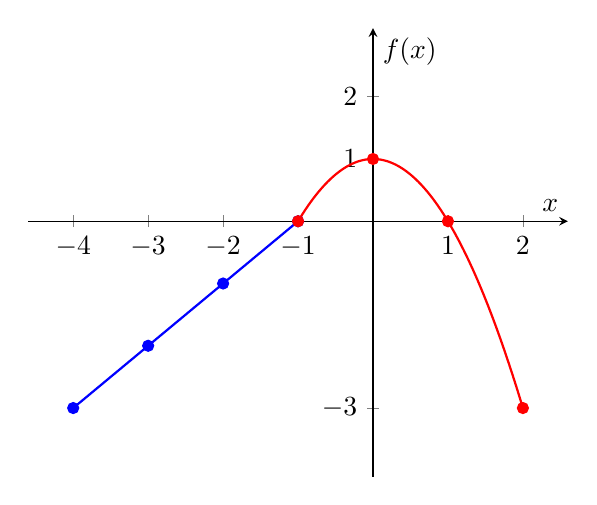
\begin{tikzpicture}
        \begin{axis}[
            axis lines = middle,
            xlabel = $x$, ylabel = {$f(x)$},
            samples=100,
            domain=-4:2,
            xtick={-4,-3,-2,-1,0,1,2}, % Marcas en X cada 1 unidad
            ytick={-3,1,2},
            ymin=-3.5, ymax=2.5,
            enlargelimits=true]

            % Primer tramo: f(x) = x+1 para -4 <= x < -1
            \addplot[blue, thick, domain=-4:-1] {x+1};  
            \addplot[blue, only marks, mark=o] coordinates {(-1,0)}; % Punto abierto en -1
            
            % Agregar puntos en cada x avanzando de 1 en 1
            \addplot[blue, only marks, mark=*] coordinates {(-4,-3) (-3,-2) (-2,-1)}; 

            % Segundo tramo: f(x) = 1 - x^2 para -1 <= x <= 2
            \addplot[red, thick, domain=-1:2] {1 - x^2};  
            \addplot[red, only marks, mark=*] coordinates {(-1,0) (0,1) (1,0) (2,-3)}; % Puntos exactos

        \end{axis}
    \end{tikzpicture}
\end{center}
    
\end{frame}

\begin{frame}{Suma superior e inferior}
    \framesubtitle{Práctica 3}

4. Sea \(f: [0,1] \to \mathbb{R}\) la función definida por:
\vspace{0.25cm}

\[f(x) = \begin{cases}
    \; x & \quad \text{si } x \notin \mathbb{Q} \\
    \; 1 & \quad \text{si } x \in \mathbb{Q}
\end{cases}\]
\vspace{0.25cm}

\((a)\) Dada una partición \(P\) cualquiera del intervalo \([0,1]\), determine la suma inferior y superior, de \(f\) asociada a la partición. \\
\vspace{0.25cm}
\((b)\) Demuestre que \(\underline{S}\leq\frac{1}{2}\), para cualquier partición. \\
\vspace{0.25cm}
\((c)\) Explique por qué \(f\) no es integrable en el intervalo \([0,1]\)

\end{frame}


\end{document}